\subsection{Опис даних}


{
Для навчання моделі та проведення експериментів використовувалися дані мононуклеарних клітин периферичної крові людини. 
Кожна клітина належить до одного із семи типів, і кожен тип містить різну кількість клітин. Клітина може належати до однієї із двох груп: контрольної (немає впливу ліків) та стимульованої (після лікування Інтерфероном (IFN$-\beta$)). Типи клітин та кількості клітин у групах такі: CD4T (2437 контрольних, 3127 стимульованих), CD4T-Mono (1946 контрольних, 615 стимульованих), B (818 контрольних, 993 стимульованих), CD8T (574 контрольних, 541 стимульованих). ), NK (517 контрольних, 646 стимульованих), F-Mono (1100 контрольних, 2501 стимульованих), Dendritic (615 контрольних, 463 стимульованих), що показано на малюнку \ref{figure-dataset-original}. 

Загальна кількість екземплярів (клітин) - 16893, з профілем експресії генів кожної клітини у 6998 генах. Більш конкретно, кожна окрема клітина представлена як одновимірний вектор довжиною 6998. Дані є публічними та були взяті з існуючого наукового дослідження [Kang]. Попередня обробка, очищення, перевірка якості, нормалізація і логарифмічна трансформація виконані згідно із найкращими практиками попередньої обробки даних, отриманих процедурою секвенування РНК [scBestPractices].


\begin{figure}[htbp]
    \centerline{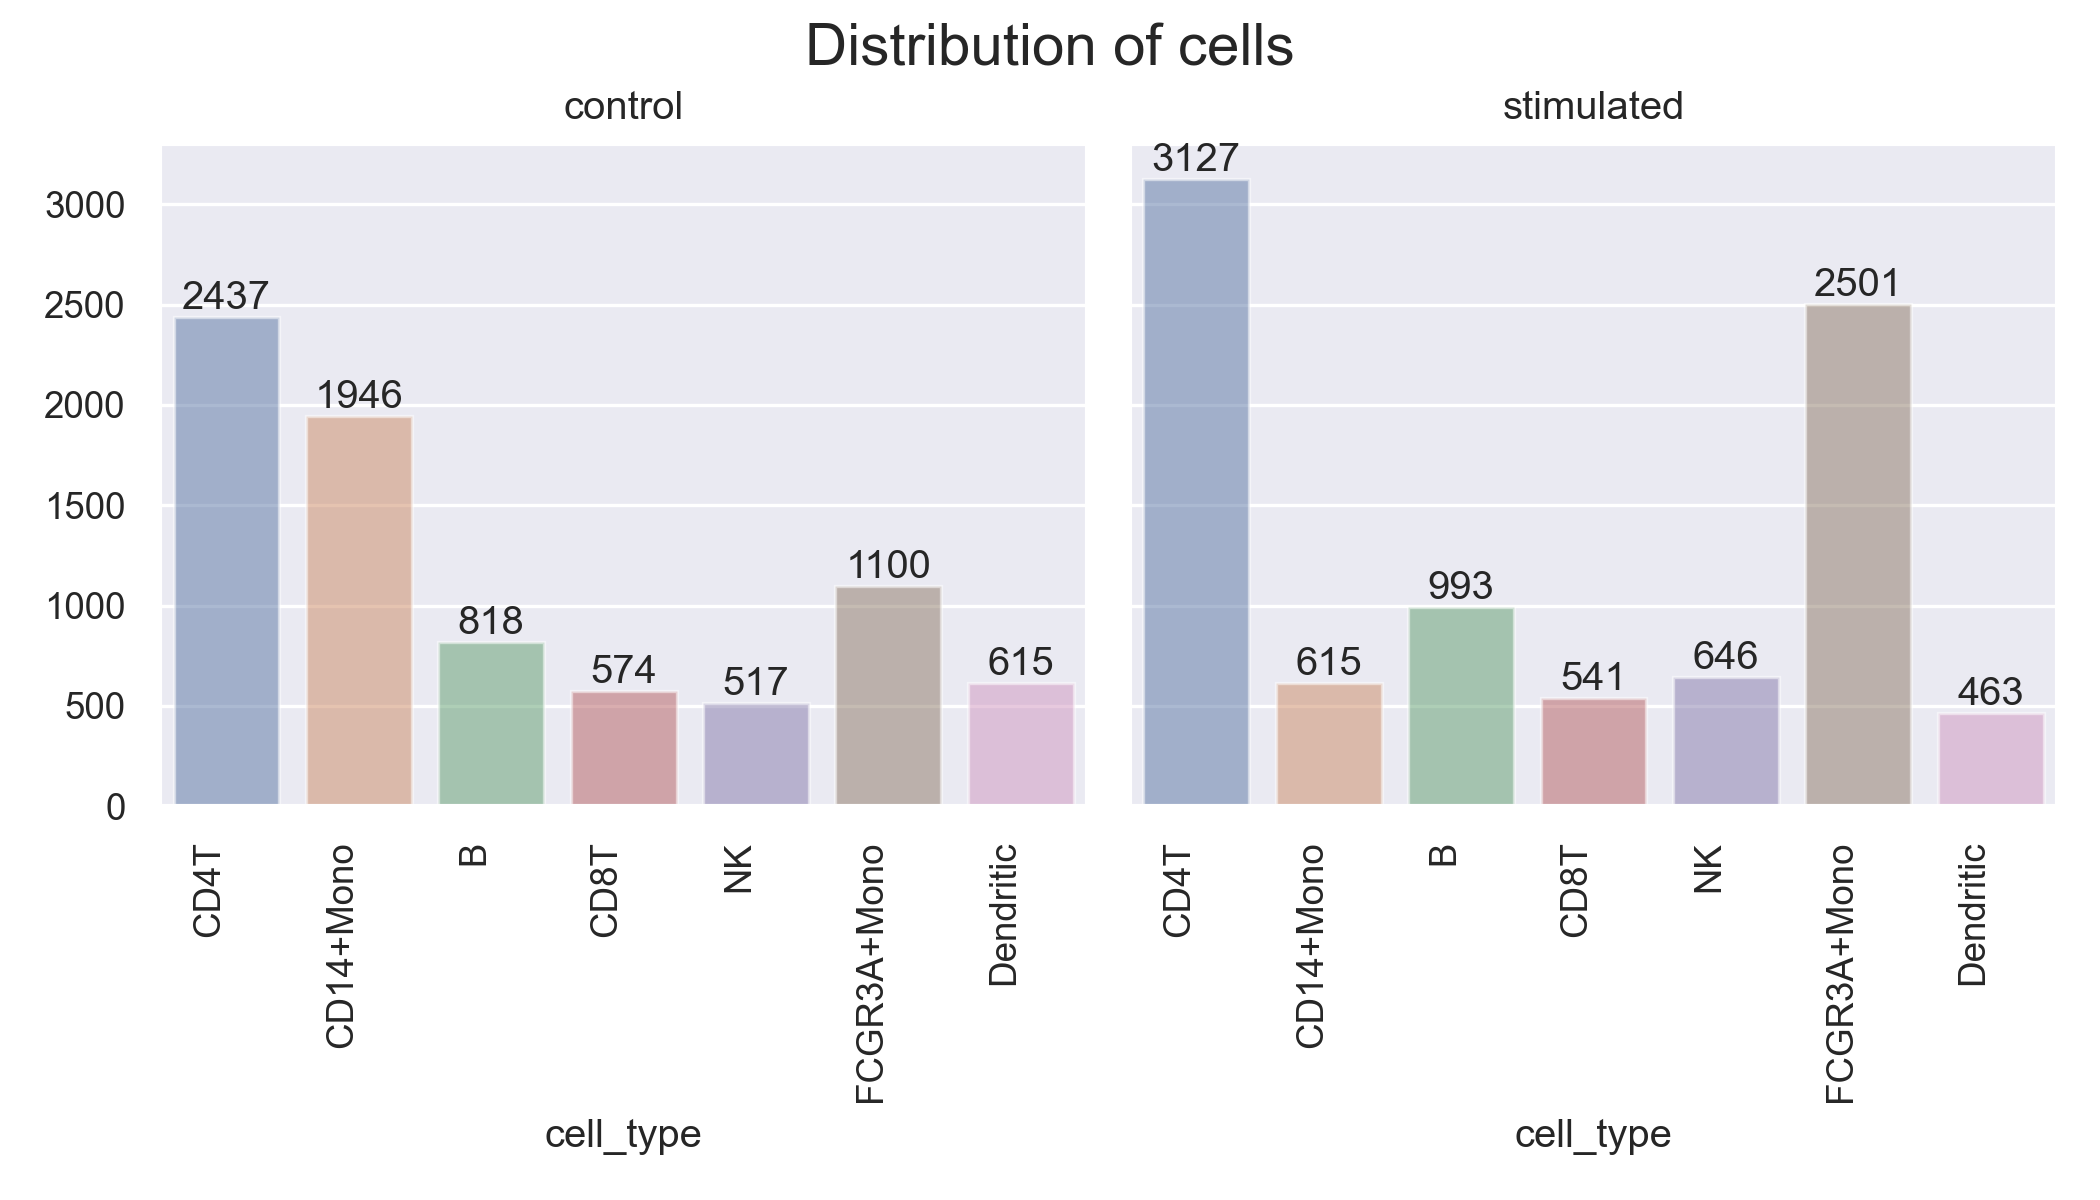
\includegraphics[width=0.6\columnwidth]{pictures/original-dataset.png}}
    \caption{Розподіл екземплярів (клітин) по типах та групах.}
    \label{figure-dataset-original}
\end{figure}

\color{red}

}